% ============================================================
% WTICG paper — ready-to-paste corrected blocks.
% Each block REPLACES the whole corresponding block in the Overleaf source
% (or is NEW where noted). See wticg/README.md for the supporting numbers.
% ============================================================

% ---- [REPLACE] Introduction, 4th paragraph -----------------------------------
% Drops the unsupported "statistically indistinguishable" claim. The cloud edge
% is small but significant (diff CI [0.2, 2.1] pp excludes 0); the thesis rests
% on the ~14 pp spread across local models being far larger than the ~1.2 pp gap.
Our results show that several local models reach quality adequate for the task. The strongest configuration, Ministral 3 8B on a consumer RTX 3060, attains free-text fidelity within about one point of the cloud reference---a small gap that is statistically detectable yet practically narrow (the cloud leads by $1.2$\,pp on BERTScore, $95\%$\,CI on the difference $[0.2, 2.1]$\,pp)---while keeping every report on-premise, and exact structured fields are near-saturated across all models. At the same time, a distinct group of local models lags by a wide margin. Because this spread across local models (roughly $14$\,pp on BERTScore) is substantially larger than the gap between the best local model and the cloud reference, the practical question for on-premise deployment is which local model to adopt rather than whether to forgo the cloud at all. The residual gap that does remain is concentrated in a few narrative fields that even the cloud reference fills imperfectly.

% ---- [REPLACE] Methodology, Models paragraph ---------------------------------
\textbf{Models.} The cloud reference is DeepSeek, selected as the best-performing cloud provider in prior work \cite{anonpipeline2026}. We deliberately selected nine local models spanning a wide range of parameter scales (4B to 21B), capturing the size--quality trade-off relevant to constrained on-premise hardware rather than evaluating a single size. Six are general-purpose instruction models (Gemma 4 E4B, Qwen3 8B, Ministral 3 8B, Llama 3.1 8B, Phi-4 14B, and gpt-oss 21B), one is an openly available DeepSeek model (DeepSeek-Coder-V2 16B), and two are cybersecurity-domain fine-tuned variants (Foundation-Sec 8B Instruct and Primus-Merged 8B), both derived from Llama 3.1 8B. Models were executed on two consumer GPUs (an RTX 3060 with 12\,GB and an RTX 5080 with 16\,GB of VRAM), assigned according to their memory requirements. Per-model chunking and decoding parameters are reported in Table~\ref{tab:chunk}.

% ---- [REPLACE] Chunk table (robust footnotes, no \footnotemark) --------------
\begin{table}[!htp]
\centering
\caption{Per-model chunking and decoding parameters (in tokens). Sizes are total parameters; Gemma 4 E4B is 4B \emph{effective} (8B total, MatFormer) and gpt-oss is a 21B mixture-of-experts (MoE).}
\label{tab:chunk}
\small
\begin{tabular}{lllrrrr}
\hline
\textbf{Model} & \textbf{Backend} & \textbf{Size} &
\shortstack{\textbf{Context}\\\textbf{window}} &
\shortstack{\textbf{Chunk}\\\textbf{budget}} &
\shortstack{\textbf{Output}\\\textbf{reserve}} &
\shortstack{\textbf{Output}\\\textbf{cap}} \\
\hline
Gemma 4 E4B             & Ollama & 4B   & 16000 & 10000 & 3000 & 2500 \\
Qwen3                   & Ollama & 8B   & 16000 & 10000 & 3000 & 2500 \\
Ministral 3             & Ollama & 8B   & 16000 & 10000 & 3000 & 2500 \\
Llama 3.1               & Ollama & 8B   & 16000 & 10000 & 3000 & 2500 \\
Phi-4                   & Ollama & 14B  & 16000 & 10000 & 3000 & 2500 \\
DeepSeek-Coder-V2       & Ollama & 16B  & 16000 & 10000 & 3000 & 2500 \\
gpt-oss                 & Ollama & 21B  & 16000 & 10000 & 3000 & 6000\textsuperscript{a} \\
Foundation-Sec Instruct & HF     & 8B   & 64K\textsuperscript{b}  & 10000 & 3000 & 2500 \\
Primus-Merged           & HF     & 8B   & 128K\textsuperscript{b} & 10000 & 3000 & 2500 \\
\hline
deepseek-v4-flash       & Cloud  & 284B & $\sim$1M\textsuperscript{b} & 10000 & 3000 & 2500 \\
\hline
\end{tabular}

\vspace{3pt}
{\footnotesize\raggedright
\textsuperscript{a}\,gpt-oss is a reasoning model; reasoning shares the output budget, so it needs a larger cap.\\
\textsuperscript{b}\,For HF and cloud models we set no context cap; the value is the architecture maximum or the API context limit.\par}
\end{table}

% ---- [REPLACE] Results opening paragraph -------------------------------------
Our central finding is that \emph{privacy-preserving, on-premise extraction is viable}: the strongest local model comes within about one point of the 284B cloud reference on free-text semantic similarity, while deterministic fields (CVSS, port, protocol, severity) and schema conformance are essentially solved even at 8B. The residual gap to the cloud is concentrated in the narrative free-text fields and in severity classification, not in structured extraction. We develop this across four axes: extraction quality (\S\ref{sec:rq1}, RQ1), operational cost (\S\ref{sec:rq2}, RQ2), domain specialization (\S\ref{sec:rq3}, RQ3), and the privacy--quality--cost trade-off (\S\ref{sec:rq4}, RQ4). All figures are means over five runs with 95\% confidence intervals; because decoding is greedy, we attribute output quality to the model rather than the GPU, so the hardware assignment affects only the cost metrics (latency, energy, VRAM).

% ---- [REPLACE] Table 2 (tab:quality) with BERTScore 95% CIs ------------------
\begin{table*}[!htp]
\centering
\caption{Per-model extraction quality (means over five runs, in \%). Bracketed values under BERTScore are 95\% bootstrap confidence intervals (per-vulnerability resampling). Omiss.\ and Halluc.\ are per-vulnerability rates ($\downarrow$: lower is better). The cloud reference (deepseek-v4-flash) is shown below the rule; the best \emph{local} model in each column is in bold.}
\label{tab:quality}
\resizebox{\textwidth}{!}{%
\begin{tabular}{lrrrrrrrr}
\hline
\textbf{Model} & \textbf{BERTScore} & \textbf{Ent.\,F1} & \textbf{Exact} & \textbf{Omiss.}$\downarrow$ & \textbf{Halluc.}$\downarrow$ & \textbf{Schema} & \textbf{Sev.\,mF1} & \textbf{Sev.\,cov} \\
\hline
Gemma 4 E4B       & \shortstack[r]{83.5\\{\scriptsize[81.8,\,86.5]}}            & 96.2 & 58.4 & 15.7 & \textbf{8.0} & 64.8 & 97.5 & 87.7 \\
Ministral 3       & \shortstack[r]{\textbf{93.0}\\{\scriptsize[92.1,\,93.9]}}   & 98.4 & 87.1 & \textbf{2.3} & 8.8 & 96.0 & 94.2 & 87.1 \\
Qwen3             & \shortstack[r]{85.0\\{\scriptsize[83.2,\,86.8]}}            & 96.8 & 70.0 & 13.5 & 8.9 & 88.1 & 93.9 & 82.1 \\
Llama 3.1         & \shortstack[r]{85.5\\{\scriptsize[83.9,\,87.0]}}            & 95.6 & 67.4 & 3.2 & 17.4 & 99.1 & \textbf{96.6} & 84.1 \\
Phi-4             & \shortstack[r]{91.0\\{\scriptsize[89.8,\,92.0]}}            & \textbf{98.8} & \textbf{90.4} & \textbf{2.3} & 8.6 & \textbf{100.0} & 95.6 & 88.8 \\
DeepSeek-Coder-V2 & \shortstack[r]{79.4\\{\scriptsize[77.6,\,81.1]}}            & 96.8 & 77.1 & 6.7 & 12.0 & 97.7 & 84.7 & 76.0 \\
gpt-oss           & \shortstack[r]{91.1\\{\scriptsize[89.5,\,92.0]}}            & 98.5 & 87.9 & 2.6 & 9.5 & 99.8 & 95.6 & \textbf{89.8} \\
Foundation-Sec    & \shortstack[r]{78.8\\{\scriptsize[76.9,\,80.7]}}            & 97.8 & 78.5 & 2.7 & 13.3 & 82.1 & 92.1 & 82.1 \\
Primus-Merged     & \shortstack[r]{85.2\\{\scriptsize[83.9,\,86.5]}}            & 96.8 & 76.4 & 6.7 & 12.1 & 99.5 & 88.4 & 79.3 \\
\hline
\textit{deepseek-v4-flash} & \shortstack[r]{\textit{94.2}\\{\scriptsize\textit{[93.8,\,94.5]}}} & \textit{99.0} & \textit{92.2} & \textit{1.3} & \textit{5.3} & \textit{100.0} & \textit{98.1} & \textit{94.1} \\
\hline
\end{tabular}}
\end{table*}

% ---- [REPLACE + NEW] RQ3 (Domain specialization) -----------------------------
\subsection{Domain specialization}\label{sec:rq3}

Table~\ref{tab:rq3} isolates security-domain fine-tuning by comparing Llama~3.1~8B against two cybersecurity fine-tunes derived from it. Both variants raise Entity~F1 over the base ($97.8$ and $96.8$ vs.\ $95.6$), confirming that domain adaptation sharpens deterministic field identification. The effect does not generalize: Foundation-Sec lowers per-vulnerability omission ($2.7$ vs.\ $3.2$) but Primus raises it ($6.7$), and neither improves free-text fidelity (BERTScore) over the base. Foundation-Sec in particular collapses schema conformance ($82.1$ vs.\ $99.1$), trading structural discipline for marginal field gains.

\begin{table}[!htp]
\centering
\caption{Domain specialization: the generalist base (Llama 3.1 8B) vs.\ two cybersecurity fine-tunes derived from it (means, \%). Bold marks the best per column; $\downarrow$ lower is better.}
\label{tab:rq3}
\small
\begin{tabular}{lrrrr}
\hline
\textbf{Model} & \textbf{BERTScore} & \textbf{Ent.\,F1} & \textbf{Omiss.}$\downarrow$ & \textbf{Schema} \\
\hline
Llama 3.1 (base)   & \textbf{85.5} & 95.6 & 3.2 & 99.1 \\
Foundation-Sec     & 78.8 & \textbf{97.8} & \textbf{2.7} & 82.1 \\
Primus-Merged      & 85.2 & 96.8 & 6.7 & \textbf{99.5} \\
\hline
\end{tabular}
\end{table}

The marginal value of cybersecurity-specific representations is thus limited: specialization helps deterministic field identification but not free-text quality or structural conformance, and for one variant it even degrades record coverage. The same limit appears at the evaluator, as we show next.

\paragraph{Robustness to the evaluation backbone.}\label{sec:securebert}
Because our free-text metric is BERTScore, we re-scored every matched (prediction, reference) pair with SecureBERT~\cite{aghaei2022securebert}, a RoBERTa model pretrained on security corpora. Since SecureBERT lacks a precomputed rescaling baseline, we compare both encoders on raw (non-rescaled) scores. The two agree closely: per-model BERTScore differs by at most $0.21$\,pp across all ten models, with no change in ranking. Divergences appear only at the field level---the largest single difference is $3.9$\,pp, on long free-text fields such as \texttt{insight} and \texttt{detection\_method}---yet 336 of 360 field cells still fall within $2$\,pp. Because the agreement holds on the raw scale and the rescaling in Table~\ref{tab:quality} is a per-model monotonic transform, the reported ranking is unaffected. A domain-specific evaluation backbone therefore adds no measurable signal here, mirroring the limited gains from domain-specific extraction models.

% ---- [NEW] BibTeX (put in sbc-template.bib) ----------------------------------
% @article{aghaei2022securebert,
%   title   = {{SecureBERT}: A Domain-Specific Language Model for Cybersecurity},
%   author  = {Aghaei, Ehsan and Niu, Xi and Shadid, Waseem and Al-Shaer, Ehab},
%   journal = {arXiv preprint arXiv:2204.02685},
%   year    = {2022}
% }

% ---- Figures (PNGs in this folder) -------------------------------------------
% \begin{figure}[!htp]\centering
%   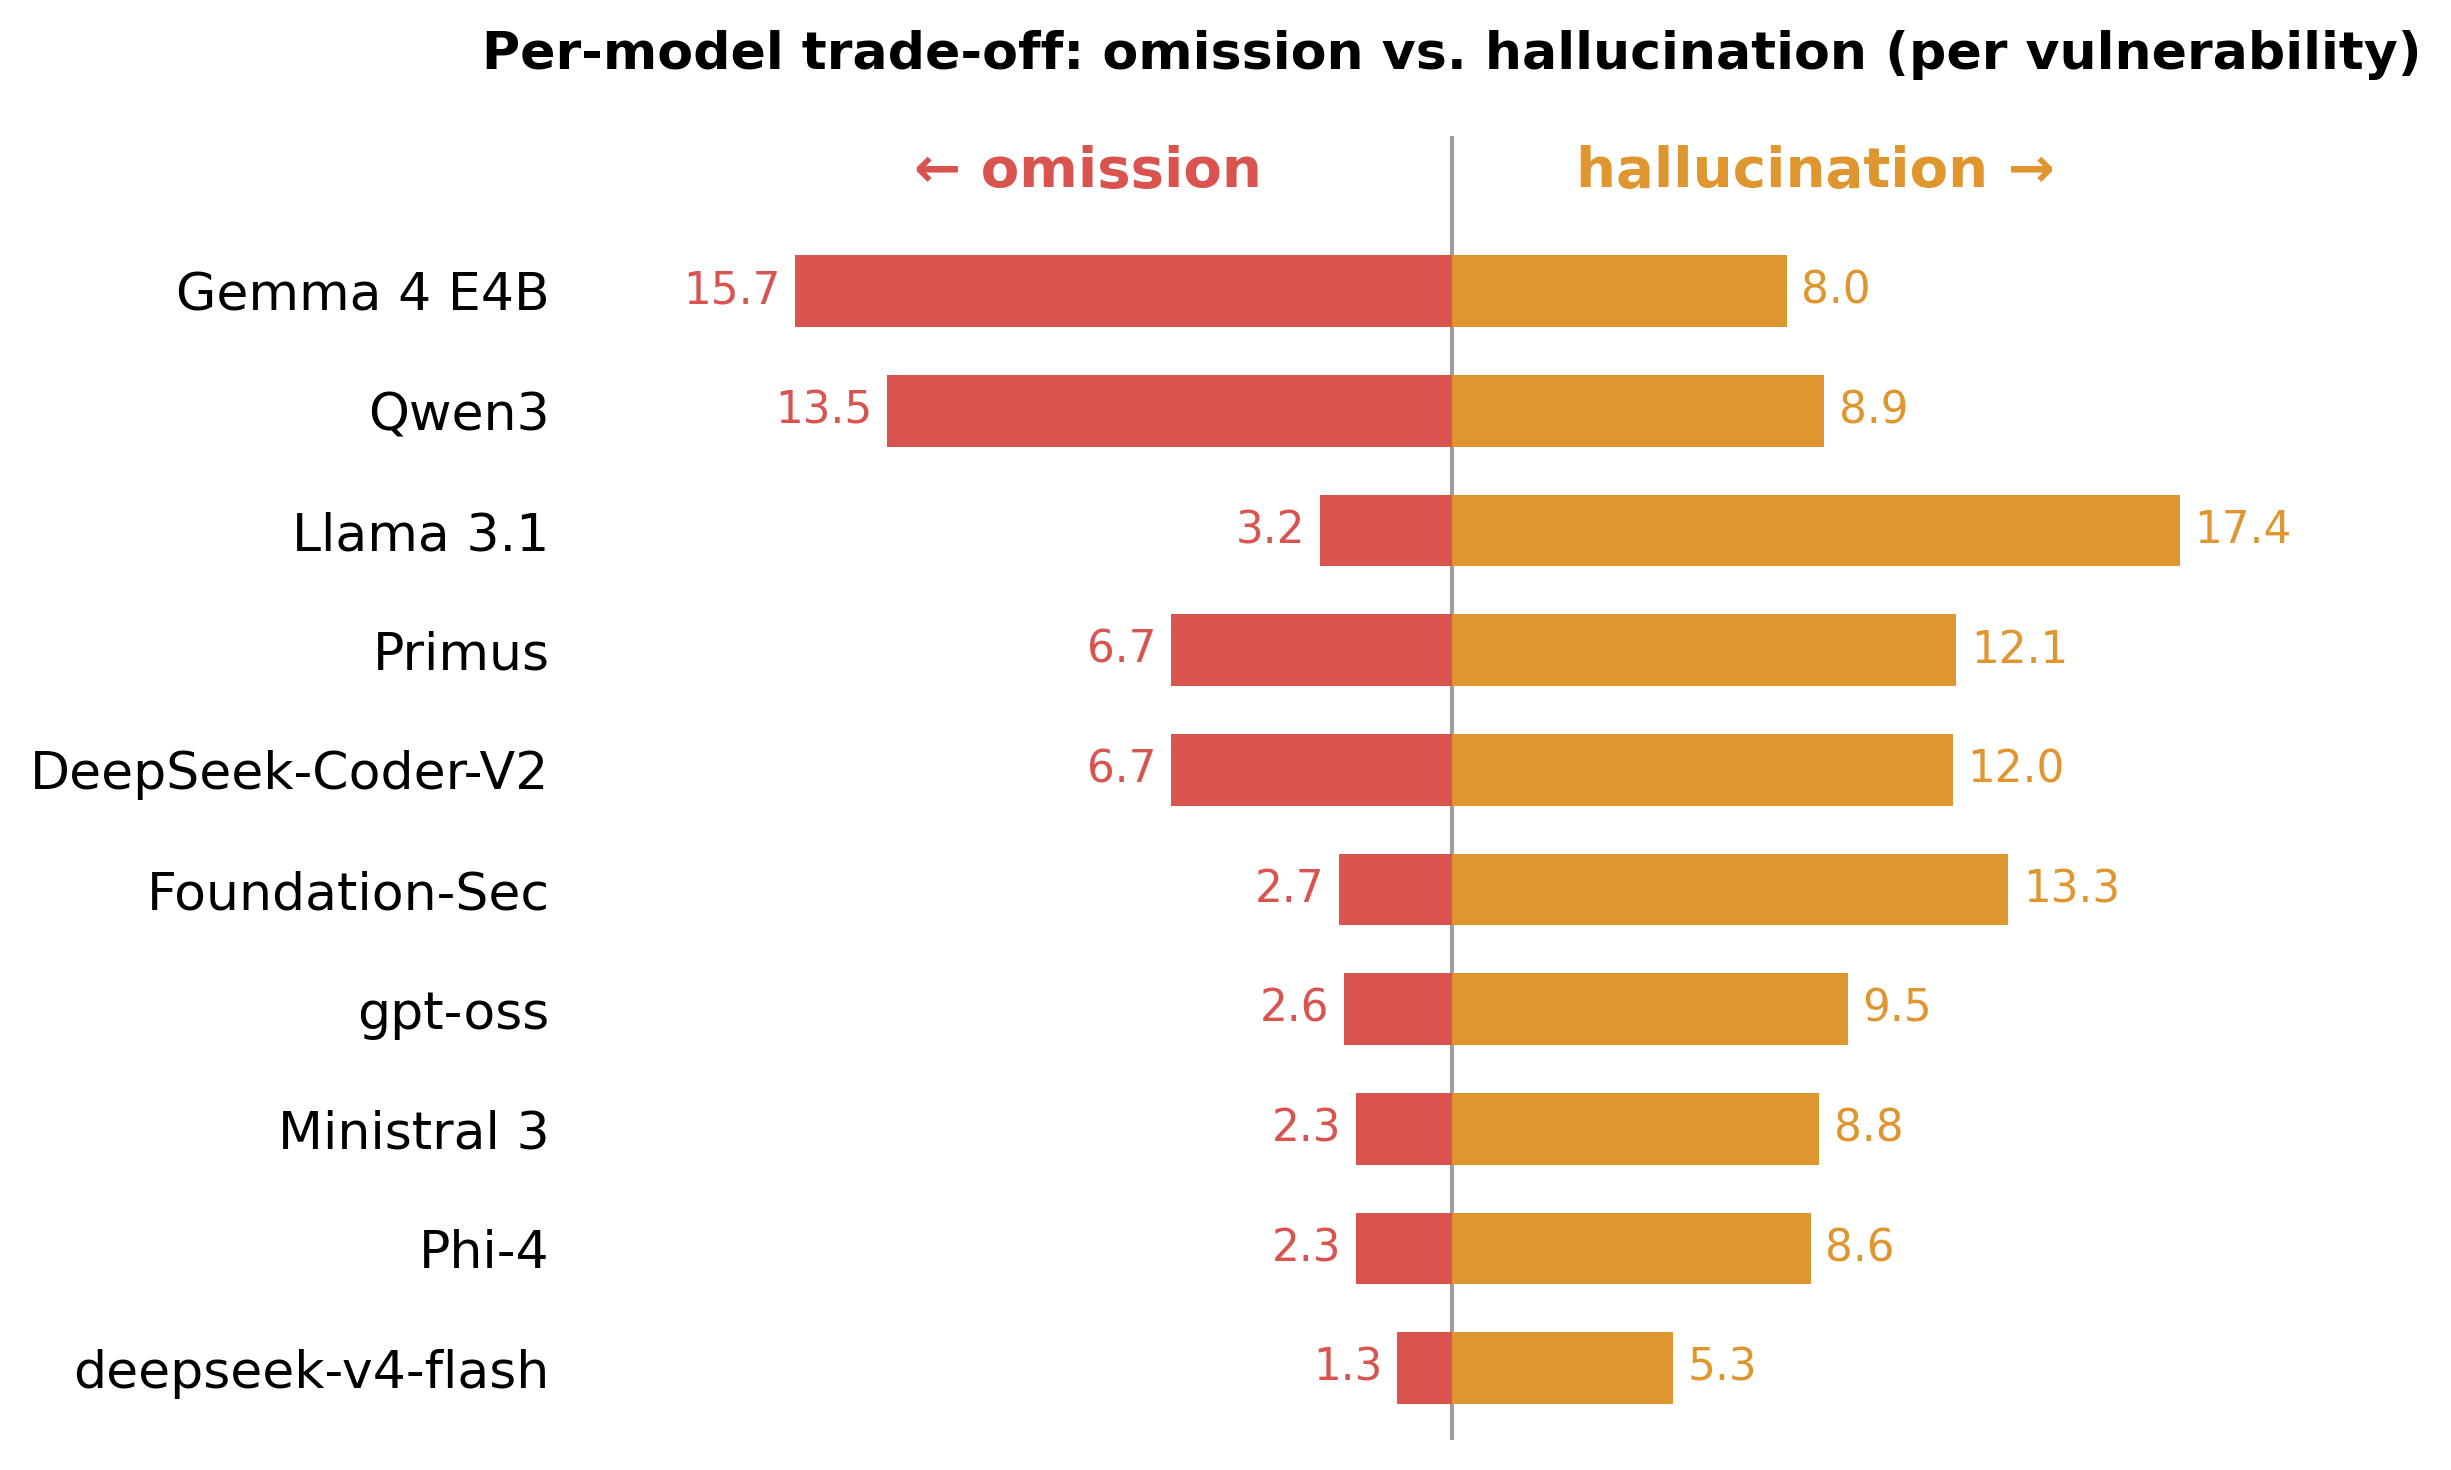
\includegraphics[width=\linewidth]{tradeoff.png}
%   \caption{Per-model trade-off between omission and hallucination (per vulnerability).}
%   \label{fig:tradeoff}
% \end{figure}
% \begin{figure*}[!htp]\centering
%   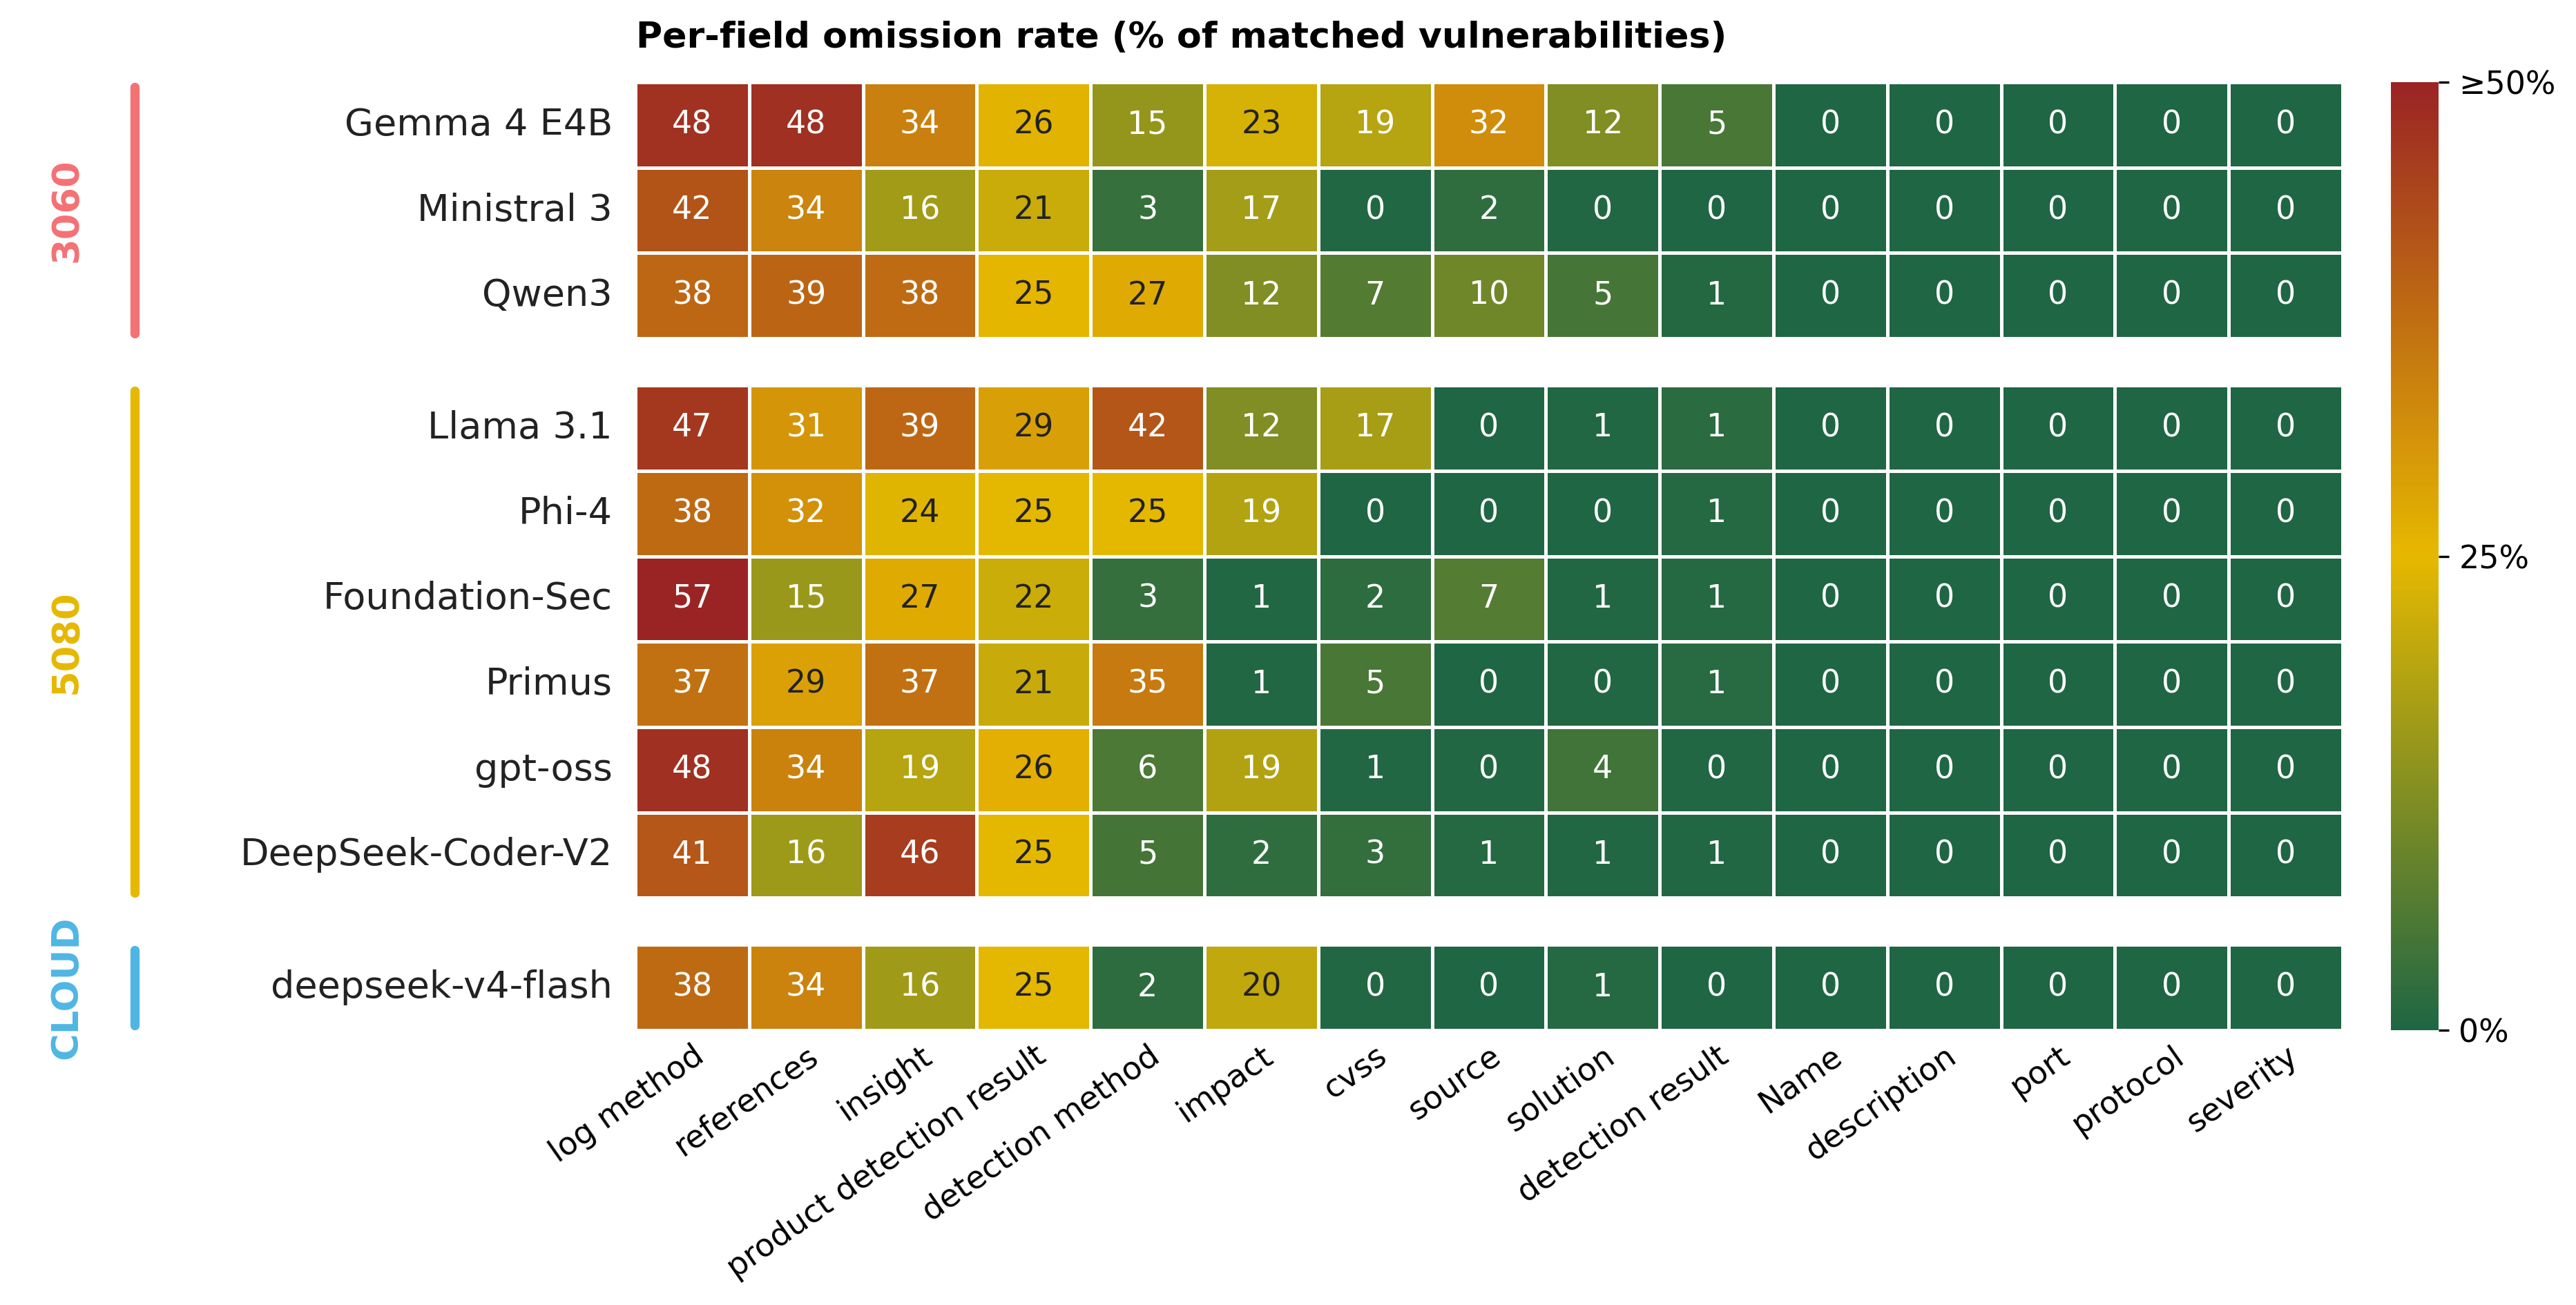
\includegraphics[width=\textwidth]{heatmap.png}
%   \caption{Per-field omission rate over matched vulnerabilities (three all-empty fields omitted).}
%   \label{fig:omission}
% \end{figure*}
